\newcommand{\LbLck}{\ensuremath{\Lb\to\Lc\Km}\xspace}
\newcommand{\LbLcpppi}{\ensuremath{\Lb\to\Lc\proton\antiproton\pim}\xspace}
\newcommand{\LbLckkpi}{\ensuremath{\Lb\to\Lc\Kp\Km\pim}\xspace}
\newcommand{\LbLcDs}{\ensuremath{\Lb\to\Lc\Dsm}\xspace}
\newcommand{\LbLcDskkpi}{\ensuremath{\Lb\to\Lc\Dsm;\Dsm\to\Kp\Km\pim}\xspace}
\newcommand{\Dskkpi}{\ensuremath{\Dsm\to\Kp\Km\pim}\xspace}


\chapter{Open-charm pentaquark search in $\Lb\to\Lc\Kp\Km\pim$ decay}
\label{chap:open_pentaquark}



\section{Study motivation}

Over the last two decades, a wealth of information has been accumulated on the decays of $b$-hadrons.
Measurements of their decays have been used to test the CKM mechanism~\cite{PhysRevLett.10.531} for describing weak decay phenomena in the Standard Model, 
as well as provide measurements against which various theoretical approaches, 
such as heavy quark effective theory ~\cite{EICHTEN1990511} and the factorization hypothesis, can be compared.
While many decays have been measured, 
a large number remain either unobserved or poorly measured, most notably decays of \Lb baryons.
LHCb has observed many new $\Lb$ decays to open charm modes, 
such as $\Lb\to\Lc\pi^-\pi^+\pi^-$~\cite{LHCb-PAPER-Define}, 
$\Lb\to\Lc \pi^- \proton \antiproton$~\cite{LHCb-PAPER-2018-005}, 
and $\Lb\to \Lc D^-_{(s)}$~\cite{LHCb-PAPER-2014-002}. 
We report the discovery of the \LbLckkpi decay in this note, where the \Lc decays to \Pp \Km \pip.
\footnote{Charge conjugate final states are implied throughout.}

Besides, 
the $\LbLckkpi$ decay also provides an opportunity to search for possible single charmed pentaquarks ($c\bar{s}uud$) 
that could decay strongly to $\Lc\Kp$.
The LHCb experiment observed two pentaquark states using $\Lb\to \jpsi p K^-$ decays in 2015~\cite{LHCb-PAPER-2015-029}.
This discovery motivates us to search for more pentaquark states.
Recently Belle reported an observation of a new $\Xic(2930)^0$ resonance decay to $\Lc\Km$ in $\Bu\to \Lc\Lcbar \Kp$ decays~\cite{Li:2017uvv}, 
and we can also examine the decays of resonances e.g. $\Xicz\to \Lc\Km$.


In the analysis of \LbLcpppi, 
the decay of \LbLckkpi has been shown as a background.
Figure~\ref{fig:feynman} shows possible contributing Feynman diagrams to the $\Lb \to \Lc \Km \Kp \pi^-$ decay.
As the knowledge about this channel is poor, the first step is  the measurement of the branching ratio.

\begin{figure}[thb]
\centering
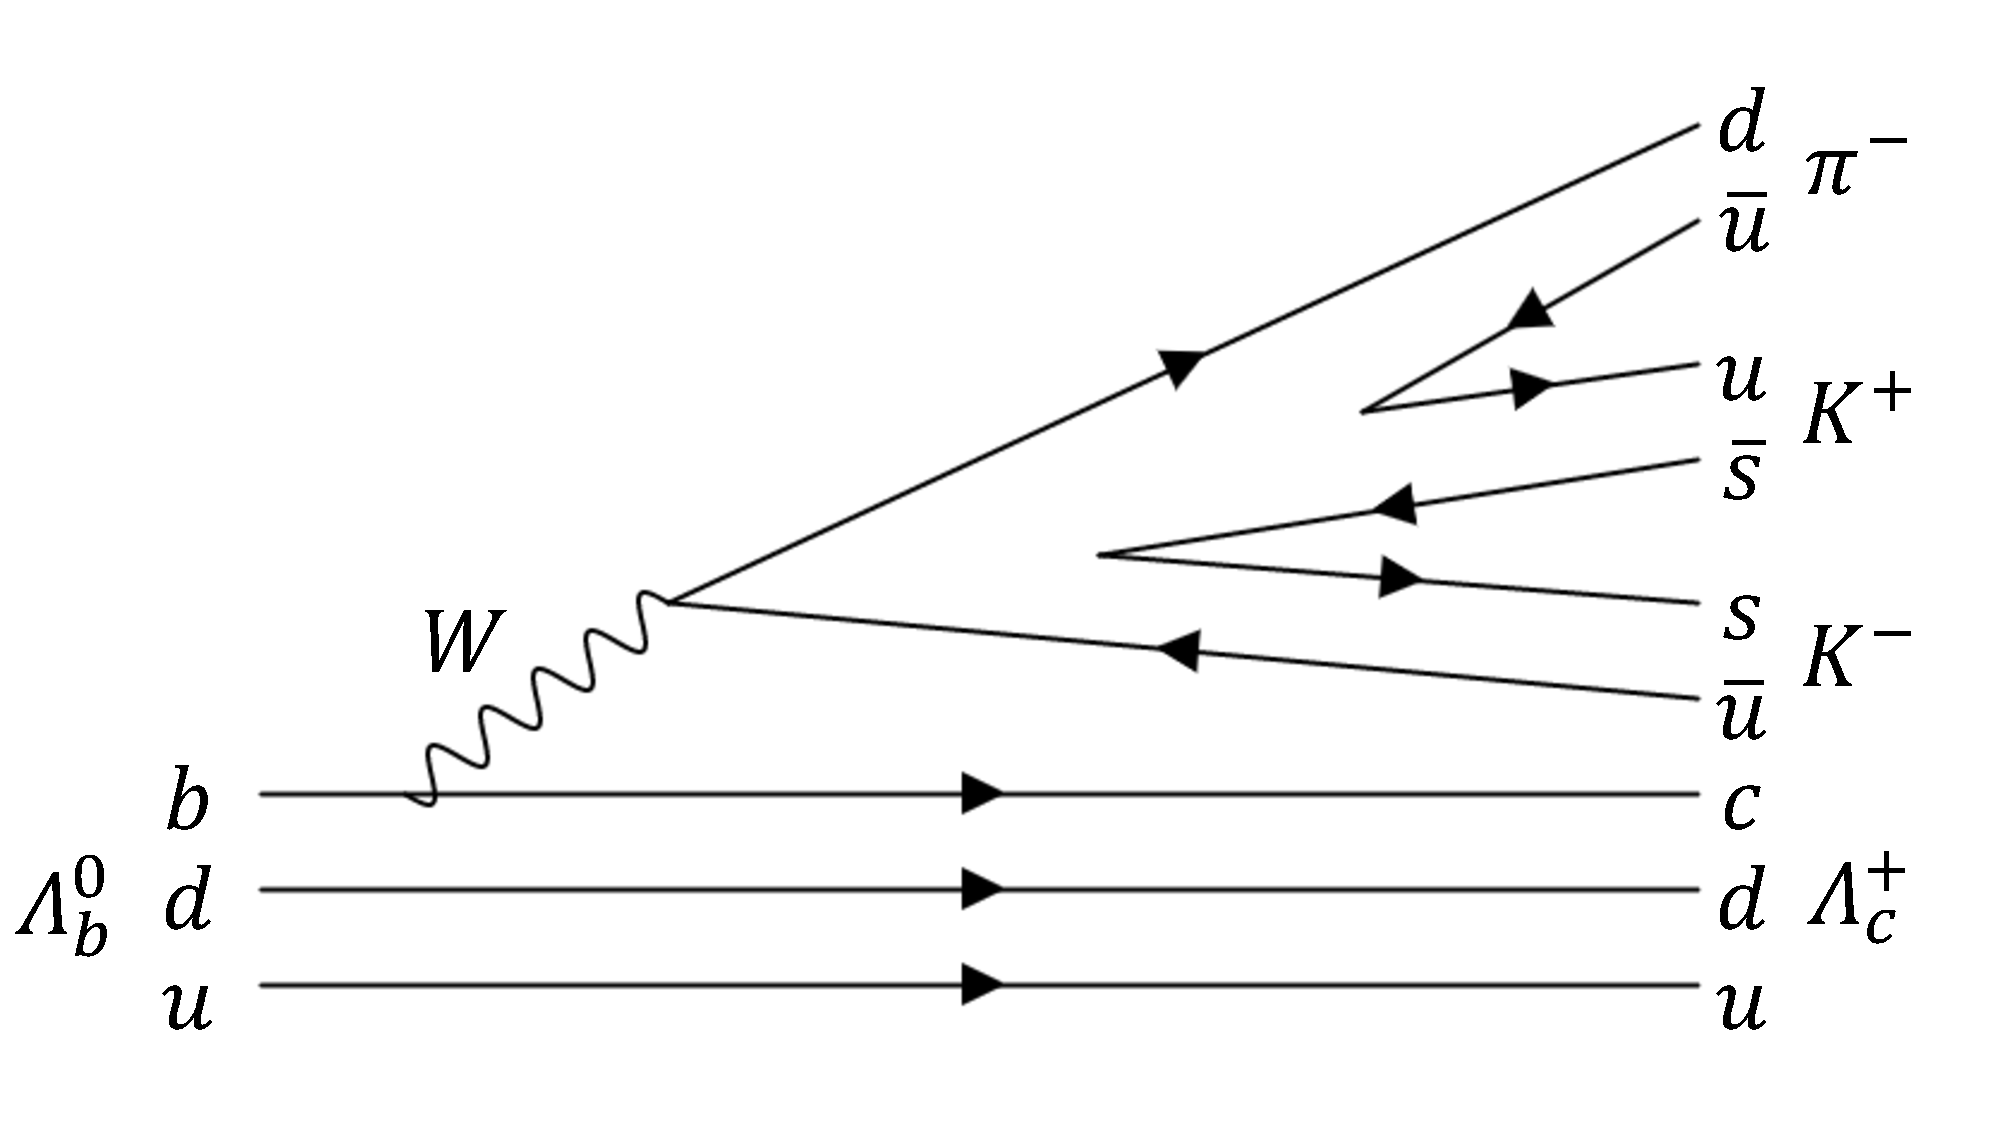
\includegraphics[width=0.6\textwidth]{Figures/05_open_charm/01_introduction/Fig1.pdf}
\caption{Possible Feynman diagrams contributing to the decay of $\Lb\to\Lc\Km\Kp\pi^-$.}
\label{fig:feynman}
\end{figure}

The branching fraction of the \LbLckkpi decay with respect to that of the \LbLcDs decay (with \Dskkpi), defined as
\begin{equation}
R \equiv \frac{\BR( \LbLckkpi)}{\BR( \LbLcDskkpi)}
\end{equation}
is measured in this analysis. 
The \LbLcDs(\Dskkpi) decay channel is taken as a normalization channel, 
which has identical final states as that of the signal channel to cancel large systematic uncertainties. 
The ratio is determined as
\begin{equation}
\label{eq:relativeBR}
\begin{split}
	R &= \frac{\BR( \LbLckkpi)}{\BR( \LbLcDskkpi)} \\
        &=\frac{N(\LbLckkpi)}{N(\LbLcDskkpi)}\,\frac{\epsilon(\LbLcDskkpi)}{\epsilon(\LbLckkpi)},
\end{split}
\end{equation}
by measuring the numbers ($N$) of candidates from signal and normalization modes 
and the relative efficiency ($\epsilon$) between the \LbLckkpi and \LbLcDs(\Dskkpi) decays.










